% !TeX root=main.tex
\chapter{تعاریف و مفاهیم مبنایی}
\thispagestyle{empty}

\section{تعبیه کلمات \protect \footnote{\lr{word embedding}}}
	بیشتر الگوریتم‌های یادگیری ماشین و یادگیری عمیق  قادر به پردازش متن به شکل خام وساده نیستند  و برای بازنمایی متن‌ها نیاز به تعبیه کلمات دارند. تعبیه کلمات نگاشت کلمات یا عبارات از واژگان به بردارهای عددی است تا کامپیوترها بتوانند به راحتی آن‌ها را پردازش کنند. تعبیه کلمات عمدتاً برای مدل‌سازی زبان و یادگیری ویژگی در پردازش زبان طبیعی استفاده می‌شود. ایده اصلی در پشت تمام روش‌های تعبیه کلمات، گرفتن هرچه بیشتر اطلاعات معنایی و ریخت‌شناسی است. روش‌های تعبیه کلمات بسیاری در مسئله پرسش و پاسخ تصویری استفاده شده است. در ادامه به برجسته‌ترین و پرکاربردترین روش‌های تعبیه کلمات موجود و استفاده‌شده در مسئله پرسش و پاسخ تصویری می‌پردازیم و معایب و مزایای هر کدام را بررسی خواهیم کرد.
\subsection{کدگذاری \lr{one-hot}}
	روش کدگذاری
	\lr{one-hot}
	ساده‌ترین روش تعبیه کلمات است. در این روش یک لغت‌‌نامه از همه واژه‌های منحصربه‌فرد موجود در مجموعه‌داده ساخته‌می‌شود و اندیس یکتایی به هر واژه اختصاص می‌یابد. بنابراین برای هر واژه یک بردار به طول تعداد واژ‌ه‌ها ساخته می‌شود که تمامی مقادیر آن صفر است به جز اندیس مربوط به همان واژه که مقدار آن یک است. پیاده‌سازی این روش آسان است اما طول بردارها  بزرگ است زیرا برابر با تعداد کل واژه‌های منحصر به فرد مجموعه داده است و هزینه زیادی برای ذخیره‌سازی دارد. بزرگترین عیب این روش  این است که نمی‌توان از آن معنا  و مفهوم استخراج کرد زیرا فاصله‌ی تمامی کلمات با هم یکسان است. در صورتی که ما انتظار داریم؛ کلماتی که مشابه هم هستند بردارهای نزدیک به هم یا مشابه هم داشته باشند و کلملاتی که معنای متفاوتی با یکدیگر دارند تا حد امکان بردارهایشان از هم دور باشند. 

\subsection{\lr{CBOW}‌ و \lr{Skip-gram}}
	برای رفع مشکلات کدگذاری 
	\lr{one-hot}
	، دو روش
	\lr{CBOW} 
	\footnote{\lr{Continouse Bag Of Words}}
	\cite{mikolov2013efficient}
	و
	\lr{Skip-gram}
	\cite{mikolov2013efficient}
	پیشنهاد شد که از شبکه‌های عصبی به عنوان جز اصلی خود استفاده می‌کنند. این دو مدل بر عکس هم کار می‌کنند.	در هر دو مدل، از یک شبکه عصبی سه لایه که شامل لایه ورودی، لایه پنهان ولایه خروجی است، استفاده شده است. درمدل 
	\lr{CBOW} 
	کلمات اطراف و نزدیک به یک کلمه(\lr{n-1}کلمه) به لایه ورودی داده می‌شود و مدل سعی می‌کند این کلمه (\lr{n}امین کلمه) را حدس بزند.  بعد از آموزش این شبکه‌، وزن بین لایه‌ی پنهان و لایه خروجی، کلمات مجموعه داده را بازنمایی می‌کند که هر ستون آن بردار مربوط به یک کلمه را نشان می‌دهد. در مدل
	\lr{skip-gram}
	برعکس 
	\lr{CBOW} 
	یک کلمه به شبکه ورودی داده می‌شود و شبکه باید کلمات اطراف و نزدیک به آن را حدس بزند. 
	\begin{figure}
		\centerline{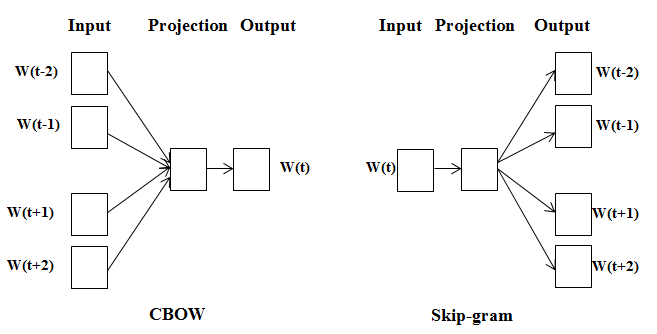
\includegraphics[scale=0.5]{images/2.png}}
		\caption{
			معماری شبکه 
			\lr{CBOW}
			و
			\lr{Skip-gram}	
		}
		\label{fig:CBOW&skip-gram}
	\end{figure}
	معماری 
	\lr{CBOW}
	و
	\lr{Skip-gram}
	در شکل 
	\ref{fig:CBOW&skip-gram}
	آورده شده است. 

\subsection{\lr{GloVe}}
	یکی دیگر از تعبیه کلمات مشهور، مدل بردار سراسری یا به اختصار 
	\lr{GloVe}
	\footnote{\lr{Global Vector}}
	است که توسط پنینگتون و همکاران 
	\cite{pennington2014glove}
	در سال 2014 در تیم پردازش زبان‌های طبیعی دانشگاه استنفورد معرفی و توسعه داده شد.
	
\subsection{\lr{CNN}‌، \lr{LSTM}‌‌و \lr{GRU}}
	با پیشرفت یادگیری عمیق در دهه اخیر، محققان برای استخراج ویژگی و بازنمایی متن از
	\lr{CNN}
	،
	\lr{LSTM}
	\footnote{\lr{Long Short-Term Memory}}
	\cite{hochreiter1997long}
	و
	\lr{GRU}
	\footnote{\lr{Gated Recurrent Unit}}
	\cite{cho2014learning}
	استفاده کردند. در مسئله پرسش و پاسخ تصویری برای استخراج ویژگی از سوال با استفاده از 
	\lr{CNN}
	بردارهای کلمات سوال در کنار هم قرار داده می‌شود سپس به لایه‌های کانولوشنی یک بعدی داده می‌شود و فیلتر‌های متفاوتی بر روی آن‌ها اعمال می‌شود و پس از عبور از لایه‌ 
	\lr{max-pooling}
	ویژگی‌ها بدست می‌آید.
	
	توضیح 
	\lr{LSTM}
	لازمه؟
	
	توضیح 
	\lr{GRU}
		لازمه؟
